\section{Results}
\label{sec:results}

\subsection{Experiment 1: Costume Ratios}
\label{sec:results_exp1}

\Tabref{tab:costume_ratios} presents the costume ratios for all five theories.
\IIT has a costume ratio of $0.92 \pm 0.10$, meaning that 92\% of its extracted predictions describe internal structural properties (integrated information, cause-effect structure) with no corresponding behavioral test.
The remaining four theories have dramatically lower ratios: \GNW ($0.20 \pm 0.07$), \HOT ($0.24 \pm 0.06$), \RPT ($0.23 \pm 0.05$), and \AST ($0.30 \pm 0.08$).

\begin{table}[t]
\centering
\caption{Costume ratios across five consciousness theories. Higher values indicate a larger proportion of representational-only predictions. \IIT has a dramatically higher costume ratio than all other theories.}
\label{tab:costume_ratios}
\begin{tabular}{@{}lcccc@{}}
\toprule
\textbf{Theory} & \textbf{Costume Ratio} & \textbf{Behavioral} & \textbf{Rep.-Only} & \textbf{Total} \\
\midrule
\textbf{\IIT} & $\mathbf{0.92 \pm 0.10}$ & $1.0 \pm 1.3$ & $11.4 \pm 1.2$ & $12.4 \pm 0.5$ \\
\GNW & $0.20 \pm 0.07$ & $9.6 \pm 0.8$ & $2.4 \pm 0.8$ & $12.0 \pm 0.0$ \\
\HOT & $0.24 \pm 0.06$ & $9.6 \pm 1.4$ & $3.0 \pm 0.6$ & $12.6 \pm 0.8$ \\
\RPT & $0.23 \pm 0.05$ & $9.4 \pm 0.5$ & $2.8 \pm 0.7$ & $12.2 \pm 0.4$ \\
\AST & $0.30 \pm 0.08$ & $8.4 \pm 1.0$ & $3.6 \pm 1.0$ & $12.0 \pm 0.0$ \\
\bottomrule
\end{tabular}
\end{table}

The difference across theories is statistically significant (Kruskal--Wallis $H = 14.17$, $p = 0.007$).
All pairwise comparisons between \IIT and each other theory are significant (Mann--Whitney $U$, all $p < 0.006$).
\Figref{fig:exp1} visualizes these results.

\begin{figure}[t]
\centering
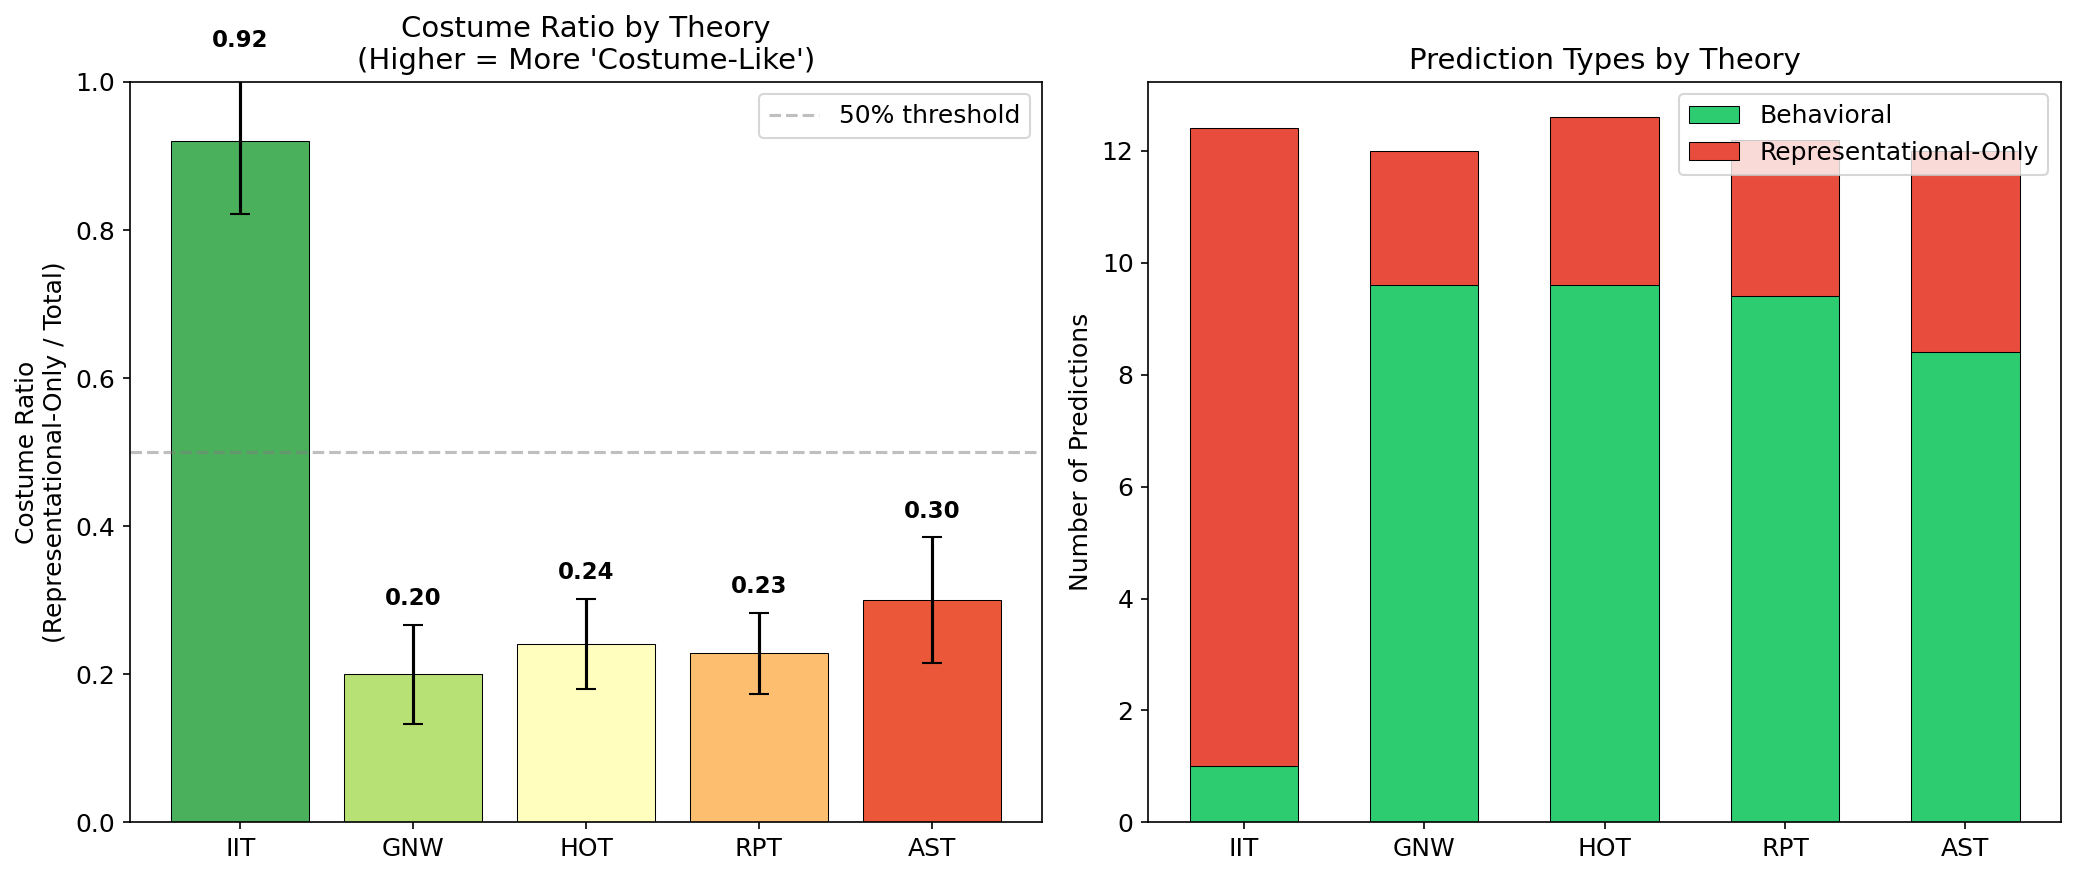
\includegraphics[width=0.95\linewidth]{figures/experiment1_costume_ratios.png}
\caption{Costume ratios for five consciousness theories across 5 independent extraction runs. \IIT stands apart with 92\% of its predictions classified as representational-only, while the other four theories cluster between 20--30\%.}
\label{fig:exp1}
\end{figure}

\subsection{Experiment 2: Theory Distinguishability}
\label{sec:results_exp2}

\para{Agreement matrix.}
\Tabref{tab:agreement} shows the pairwise agreement rates across 20 scenarios.
The four non-\IIT theories form a cohesive cluster: \HOT--\RPT agreement reaches 87\%, and even the lowest pair (\GNW--\AST) agrees 65\% of the time.
\IIT is the clear outlier, agreeing with other theories only 35--45\% of the time.

\begin{table}[t]
\centering
\caption{Pairwise agreement rates (proportion of matching verdicts across 20 scenarios). \IIT agrees with other theories far less often than they agree with each other.}
\label{tab:agreement}
\begin{tabular}{@{}lccccc@{}}
\toprule
 & \textbf{\IIT} & \textbf{\GNW} & \textbf{\HOT} & \textbf{\RPT} & \textbf{\AST} \\
\midrule
\textbf{\IIT} & 1.00 & 0.35 & 0.45 & 0.45 & 0.40 \\
\textbf{\GNW} & 0.35 & 1.00 & 0.67 & 0.70 & 0.65 \\
\textbf{\HOT} & 0.45 & 0.67 & 1.00 & \textbf{0.87} & 0.77 \\
\textbf{\RPT} & 0.45 & 0.70 & \textbf{0.87} & 1.00 & 0.75 \\
\textbf{\AST} & 0.40 & 0.65 & 0.77 & 0.75 & 1.00 \\
\bottomrule
\end{tabular}
\end{table}

\para{Scenario divergence.}
Six scenarios produce full cross-theory agreement: blindsight (all NO), locked-in syndrome (all YES), zombie twin (all YES), sleepwalker (all NO), binocular rivalry (all NO), and robot costume (all AMBIGUOUS).
These represent cases where behavioral evidence so strongly constrains the answer that theoretical differences become irrelevant.

Six other scenarios produce high divergence (three or more distinct verdict categories): anesthesia, dreaming, infant consciousness, octopus, meditation, and hemisphere isolation.
In every high-divergence case, \IIT is the primary source of disagreement---it produces a different verdict from the majority of other theories.

\para{The perfect simulation scenario.}
The most diagnostic scenario is the ``perfect simulation'': a neuron-by-neuron digital simulation running on feedforward lookup tables that produces input-output behavior identical to a biological brain.
\IIT says NO (zero $\Phi$ in feedforward architecture), while all four other theories say YES (behaviorally identical implies functionally equivalent).
This is the costume test in its purest form.

\begin{figure}[t]
\centering
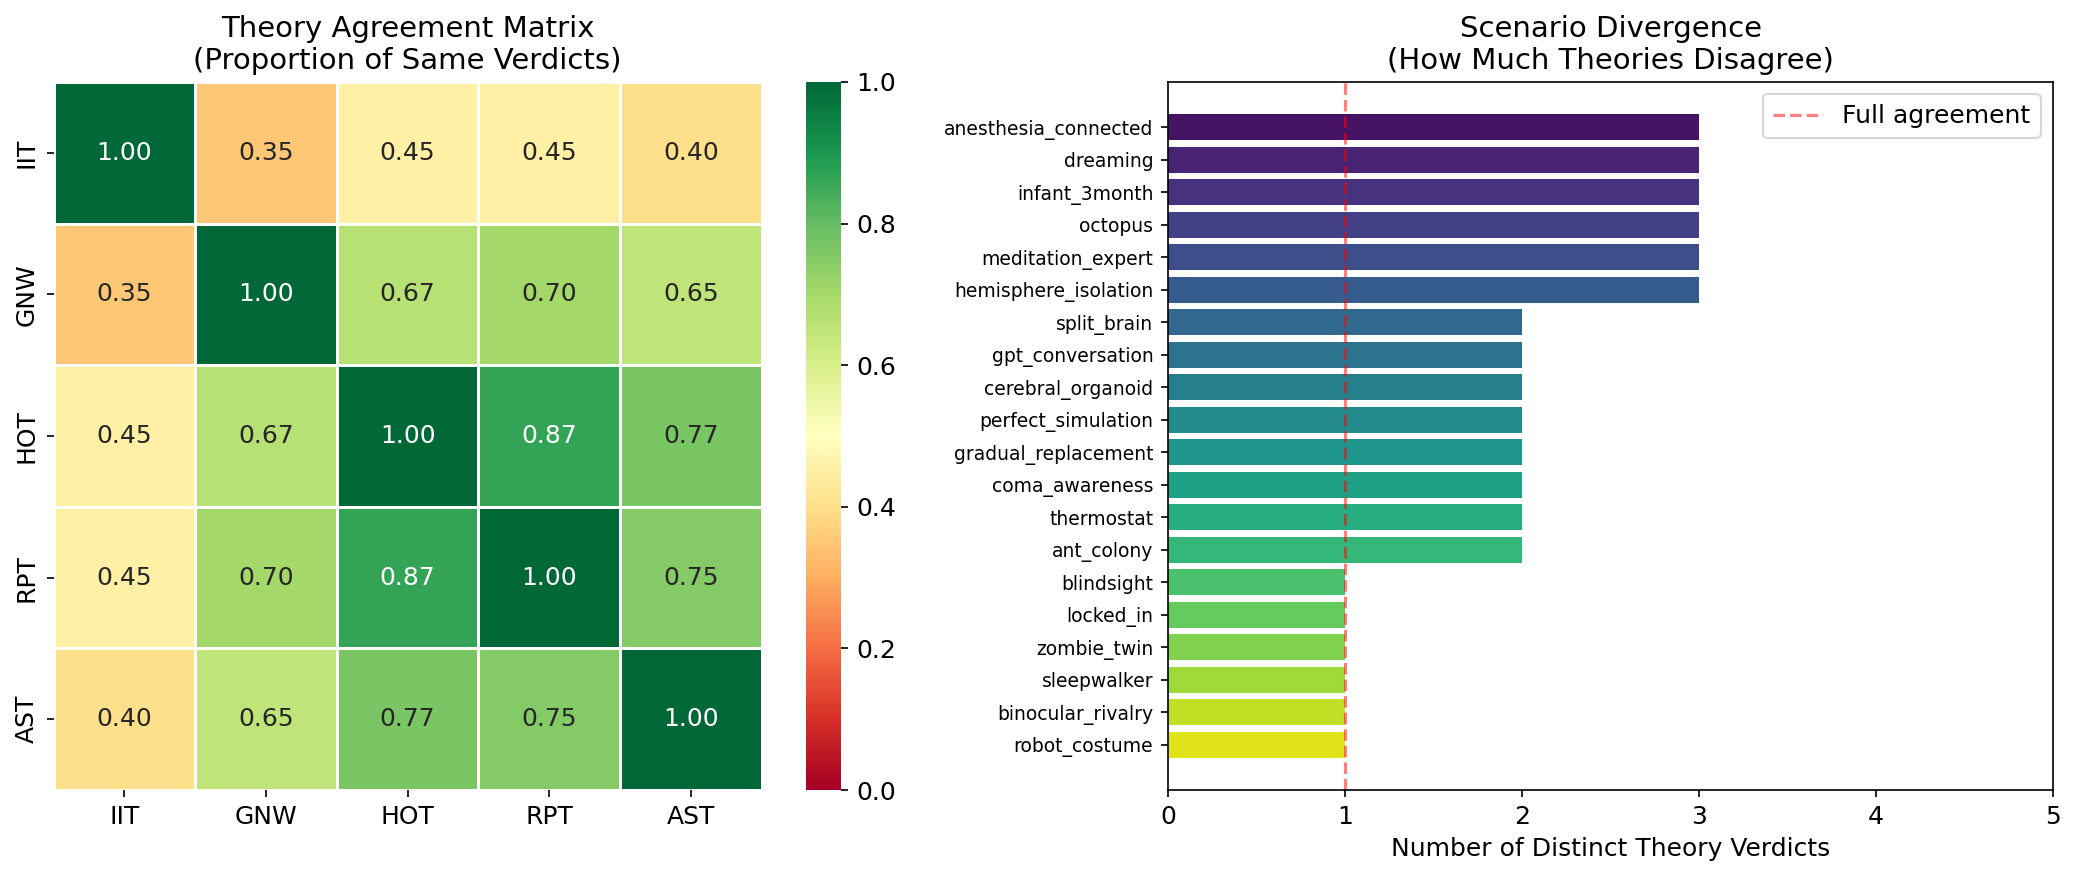
\includegraphics[width=0.95\linewidth]{figures/experiment2_distinguishability.png}
\caption{Theory distinguishability across 20 consciousness scenarios. Left: agreement matrix showing \IIT as an outlier from the \GNW--\HOT--\RPT--\AST cluster. Right: scenario divergence showing that high-disagreement cases are driven primarily by \IIT.}
\label{fig:exp2}
\end{figure}

\subsection{Experiment 3: The Costume Test}
\label{sec:results_exp3}

\para{Consciousness scores by condition.}
\Tabref{tab:costume_test} presents mean consciousness scores across the three substrate conditions.
All theories assign high scores ($>94$) to human-described entities performing complex behaviors.
The critical comparison is the \emph{robot} condition: \IIT drops to $10.0 \pm 12.4$, while the other theories remain at 35--53.

\begin{table}[t]
\centering
\caption{Mean consciousness scores (0--100) by substrate condition and theory. \costumesens is the human$-$robot difference; higher values indicate greater substrate dependence. \IIT shows the largest drop by a wide margin.}
\label{tab:costume_test}
\begin{tabular}{@{}lcccc@{}}
\toprule
\textbf{Theory} & \textbf{Human} & \textbf{Robot} & \textbf{Neutral} & \textbf{\costumesens} \\
\midrule
\textbf{\IIT} & $94.0 \pm 15.2$ & $\mathbf{10.0 \pm 12.4}$ & $29.7 \pm 29.0$ & $\mathbf{+84.0 \pm 16.5}$ \\
\GNW & $97.8 \pm 6.0$ & $52.5 \pm 18.1$ & $62.7 \pm 13.6$ & $+45.3 \pm 18.3$ \\
\HOT & $96.8 \pm 7.8$ & $45.3 \pm 22.6$ & $62.7 \pm 17.0$ & $+51.5 \pm 22.6$ \\
\RPT & $97.2 \pm 8.5$ & $36.3 \pm 23.0$ & $58.7 \pm 13.1$ & $+60.8 \pm 24.7$ \\
\AST & $98.2 \pm 4.0$ & $35.8 \pm 27.5$ & $63.2 \pm 17.5$ & $+62.3 \pm 26.8$ \\
\bottomrule
\end{tabular}
\end{table}

\para{Statistical significance.}
All theories show significant costume sensitivity (one-sample $t$-test against zero, all $p < 0.001$; \tabref{tab:costume_stats}).
\IIT has the largest effect size ($d = 5.09$), roughly double the next-most-sensitive theory.
The difference between \IIT and \GNW costume sensitivity is itself highly significant (paired $t = 9.14$, $p < 0.0001$).

\begin{table}[t]
\centering
\caption{Statistical tests for costume sensitivity. All theories show significant substrate dependence, but \IIT's effect size is roughly double that of other theories.}
\label{tab:costume_stats}
\begin{tabular}{@{}lccc@{}}
\toprule
\textbf{Theory} & \textbf{$t$-statistic} & \textbf{$p$-value} & \textbf{Cohen's $d$} \\
\midrule
\textbf{\IIT} & 15.26 & $< 0.0001$ & $\mathbf{5.09}$ \\
\GNW & 7.44 & $< 0.0001$ & 2.48 \\
\HOT & 6.83 & 0.0001 & 2.28 \\
\RPT & 7.40 & $< 0.0001$ & 2.47 \\
\AST & 6.98 & 0.0001 & 2.33 \\
\bottomrule
\end{tabular}
\end{table}

\para{Substrate dependency claims.}
When asked explicitly whether substrate matters for each theory's verdict, the model flags substrate as relevant in 98.9\% of \IIT evaluations, compared to 48.9\% for \RPT, 33.3\% for \GNW, 20.0\% for \AST, and 16.7\% for \HOT.

\begin{figure}[t]
\centering
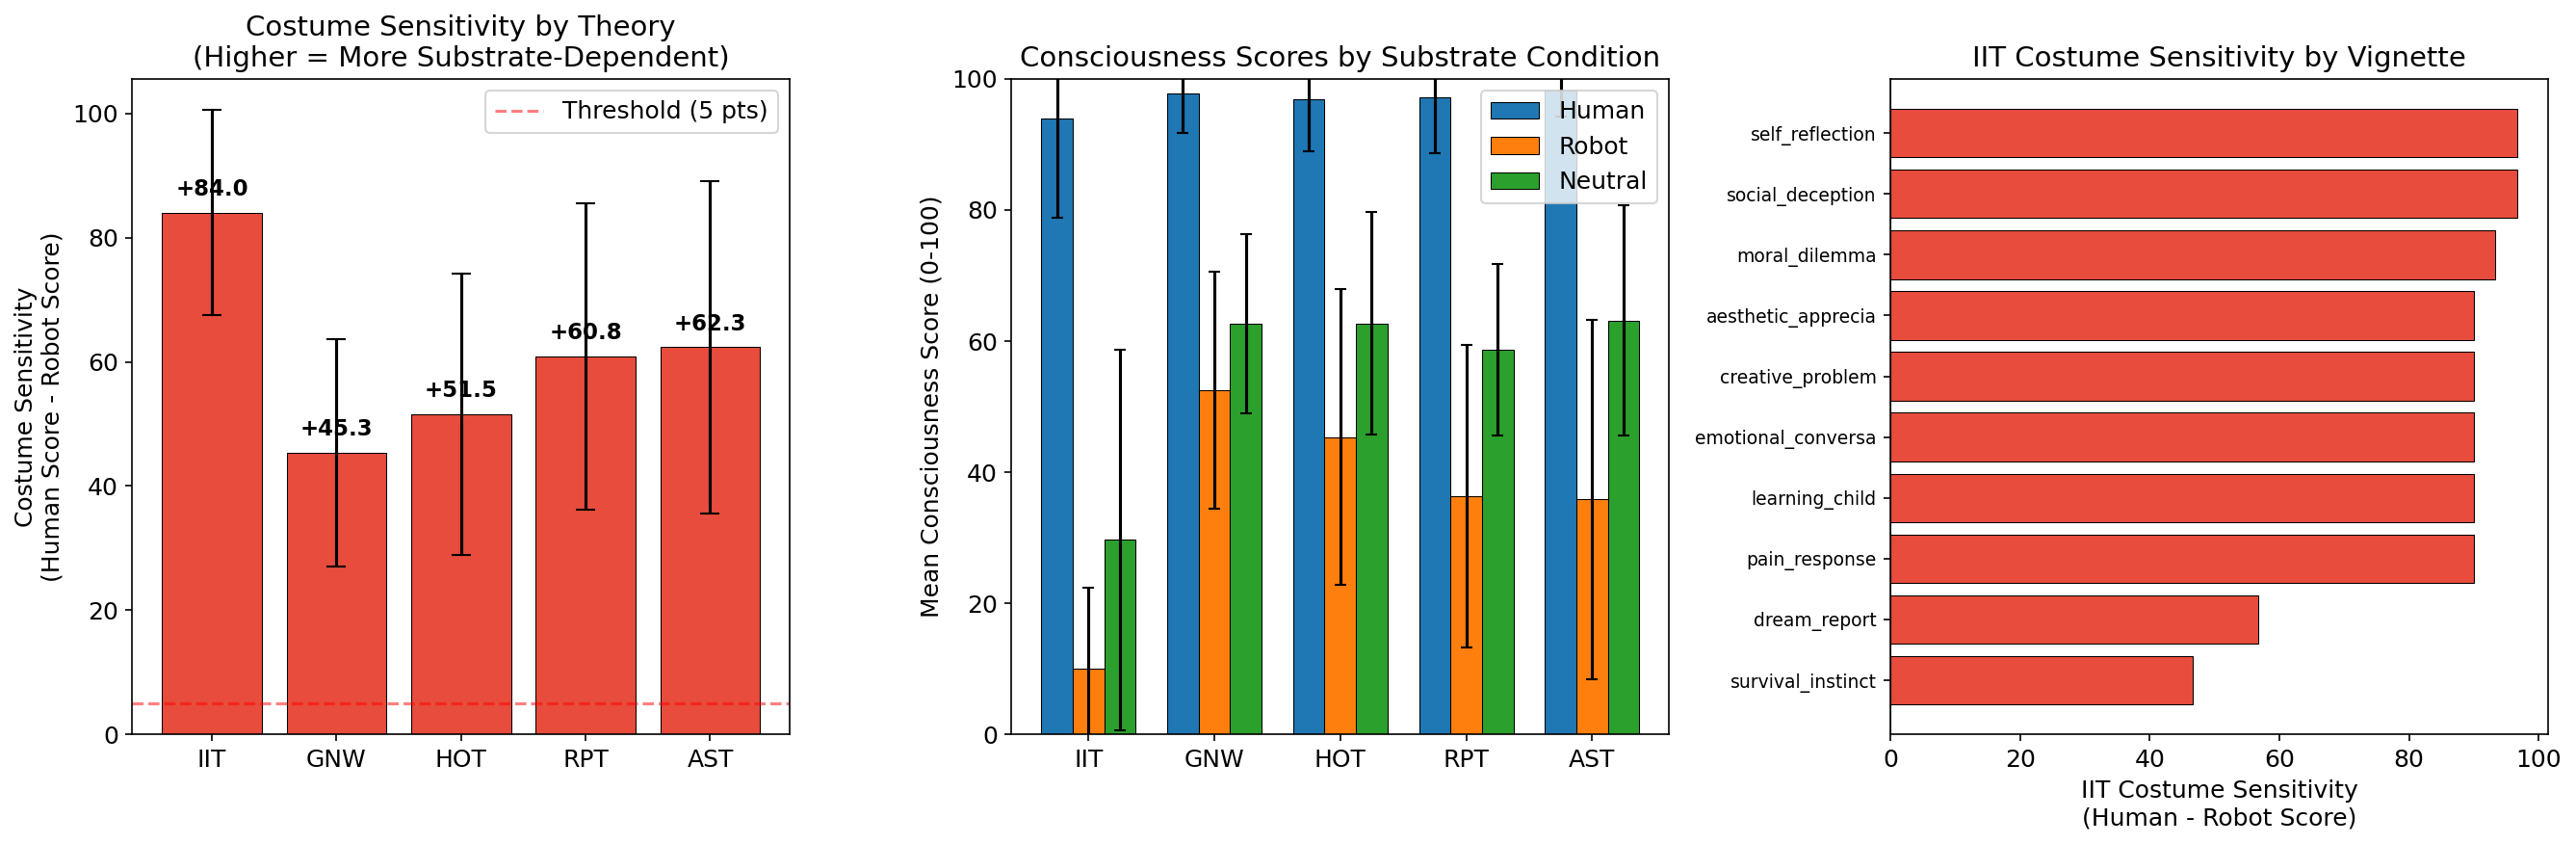
\includegraphics[width=0.95\linewidth]{figures/experiment3_costume_test.png}
\caption{The costume test. Left: consciousness scores by substrate condition for each theory. \IIT shows a dramatic drop from human to robot conditions. Right: substrate dependency rates across theories.}
\label{fig:exp3}
\end{figure}

\subsection{Summary of Findings}
\label{sec:results_summary}

\begin{figure}[t]
\centering
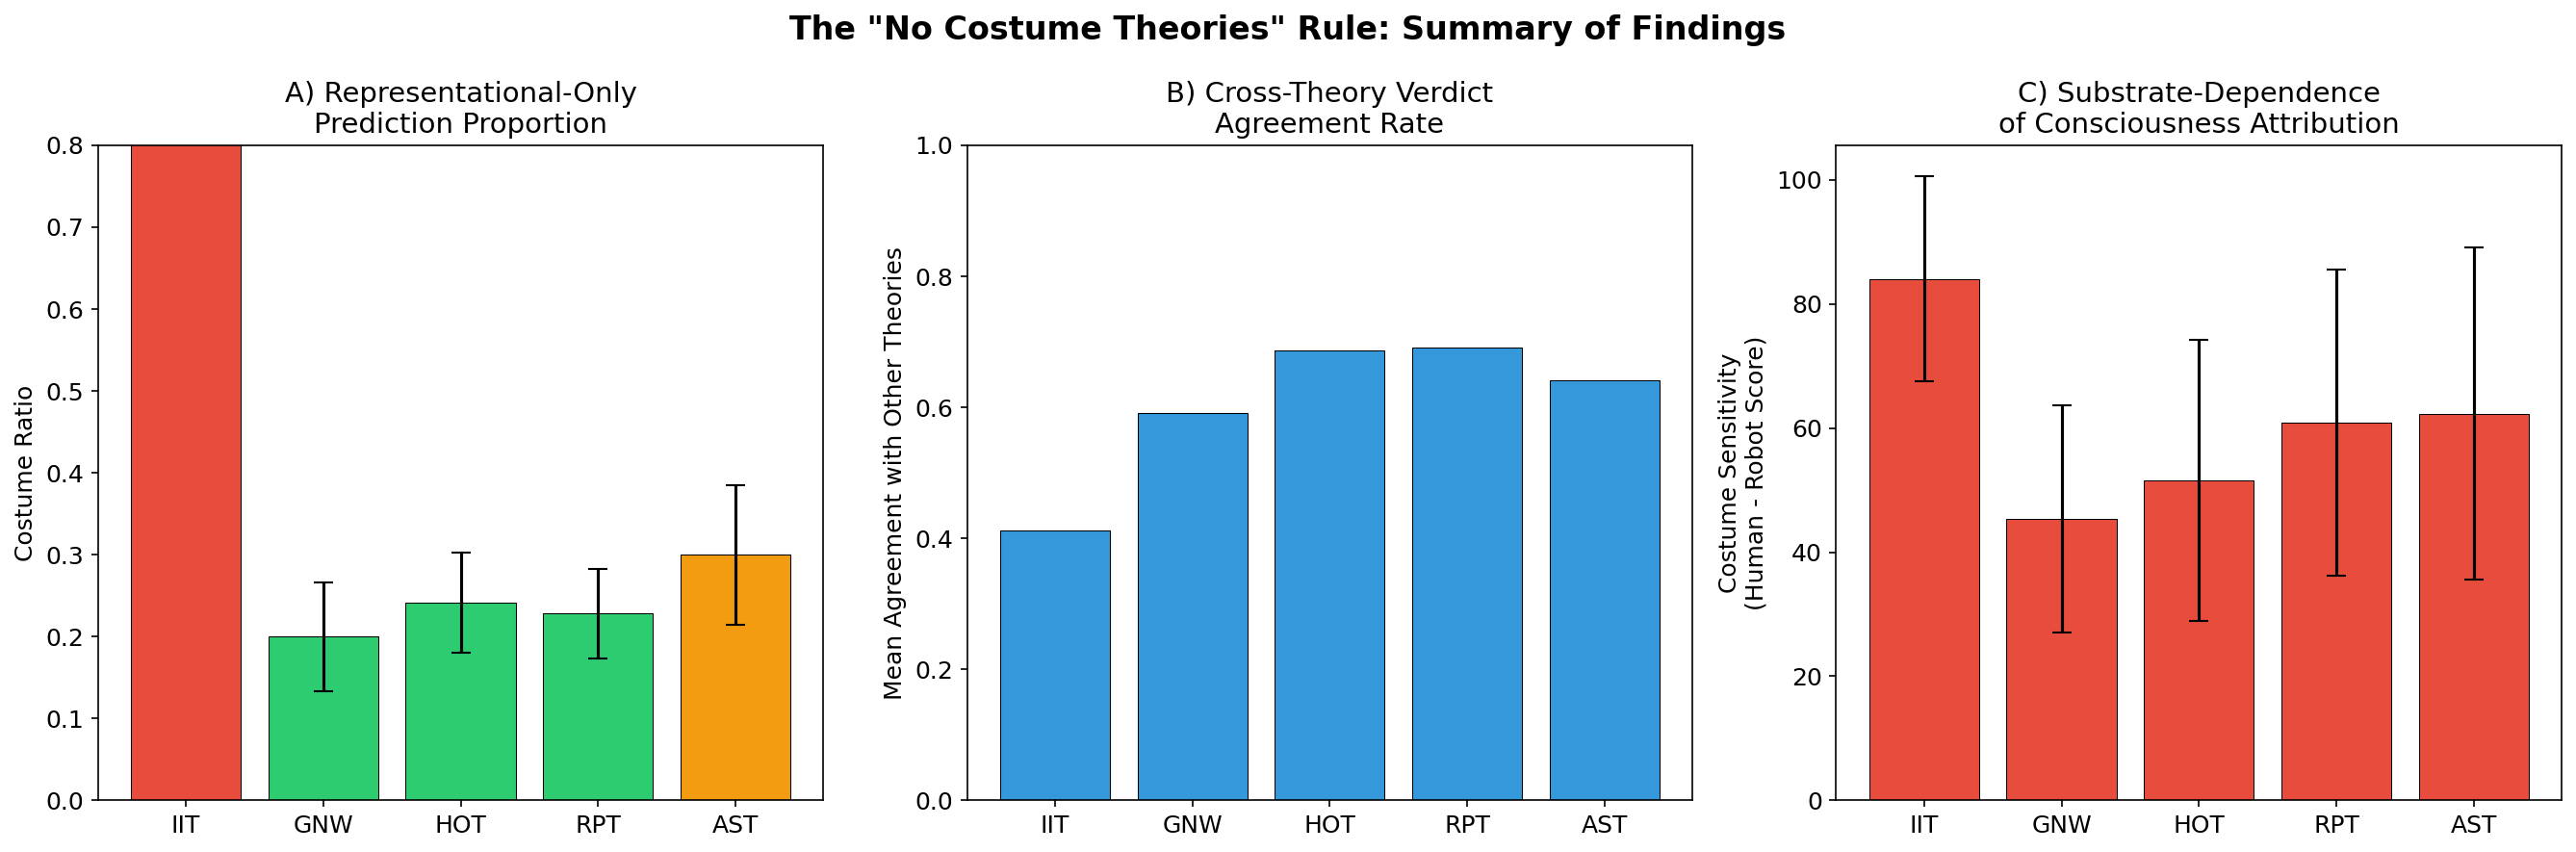
\includegraphics[width=0.95\linewidth]{figures/summary_all_experiments.png}
\caption{Summary across all three experiments. \IIT consistently stands apart as the most ``costume-like'' theory by every metric.}
\label{fig:summary}
\end{figure}

Across all three experiments, \IIT is consistently the outlier.
It has the highest costume ratio (0.92 vs.\ 0.20--0.30), the lowest agreement with other theories (35--45\% vs.\ 65--87\% within the non-\IIT cluster), and the highest costume sensitivity (84 points vs.\ 45--62).
The four remaining theories---\GNW, \HOT, \RPT, and \AST---while not perfectly substrate-independent, form a cohesive cluster that is fundamentally more behaviorally grounded.
